%!TEX root = ../Thesis.tex
\label{chapter:terminology}
\enquote{Psychophysiology is a branch of neuroscience that seeks to understand how a person's mental state and physiological responses interact to affect one another.} \cite{def_psychophysiology} For the better part of the 20th century, the concept of arousal dominated the field of psychophysiology, regardless of which physiological signal was taken into consideration \cite{cacioppo_strong_2016_p_3_15}.

In the 21st century, the advances in neurophysiological has shifted the focus to important patterns in behaviour of individual's nervous system in different situations. The demographics like individual's cultural background, social situation and interpersonal skills are considered to be powerful determinant of a person's behaviour. \cite{cacioppo_strong_2016_p_3_15}.

In this chapter, we discuss the physiological signals that will be taken into consideration for this thesis, Electrocardiogram (ECG) and Electrodermal activity (EDA). We discuss what these two physiological signals signify and measure, and why we choose them over other physiological signals.

\section{Electrocardiogram (ECG)}
The cardiovascular system of human beings consists of the heart, which is a pump and the vasculature, the distribution system that ensures that blood reaches all tissues of the body. The heart has special cardiac muscles and conducting fibers, which serve as the electrical conducting system of the heart \cite{cacioppo_cardiovascular_2016_p_183_216}.

\subsection{The Electricity of Heart} The conducting fibers cause contraction of heart muscles, the electrical charge associated that cause contraction is called 'depolarization'. The heart has four chambers. Two of four chambers of the heart contract together at a given time. Thus, from the electrical point of view the heart is considered to have two chambers \cite{hampton_ecg_2013}.

\subsection{ECG} Electrocardiography is a non-invasive method of recording the electrical activity of the heart. This is achieved by positioning leads/ electrodes on the body in a standardized location. The tiny electrical changes during a heartbeat create an electrophysiologic pattern of depolarizing and repolarizing.
\paragraph{}
The graph of the voltage of the electrical signal created during the heartbeat versus time is called ECG. Each cardiac cycle is represented by a sinus rhythm. The word 'rhythm' is referred to the part of the heart which is controlling the activation sequence. The normal heart rhythm, with electrical activation beginning in the Sinoatrial node, is called 'sinus rhythm' \cite{hampton_ecg_2013}.

\subsection{Normal Sinus Rhythm (NSR)}
A Normal Sinus Rhythm is used to denote a Sinus Rhythm of a healthy functioning heart. The Normal Sinus Rhythm (NSR) can be schematically represented in the standard waveform as showing in figure \ref{fig:sinus_rhythm_labels}. Different points on the wave are represented by a letter. The letters P, Q, R, S, and T were selected in the early days of ECG history and were chosen arbitrarily \cite{hampton_ecg_2013}. The cycle begins with the depolarization of the Sinoatrial node. The wave of the depolarization passing through the right atrial muscle corresponds to the P wave. The QRS complex of the ECG appears shortly thereafter due to atrial contraction, reflecting ventricular contraction \cite{cacioppo_cardiovascular_2016_p_183_216}. The segment between three of graphical deflections - Q, R and S points in the waveform forms a QRS Complex.

\begin{figure}
    \centering
    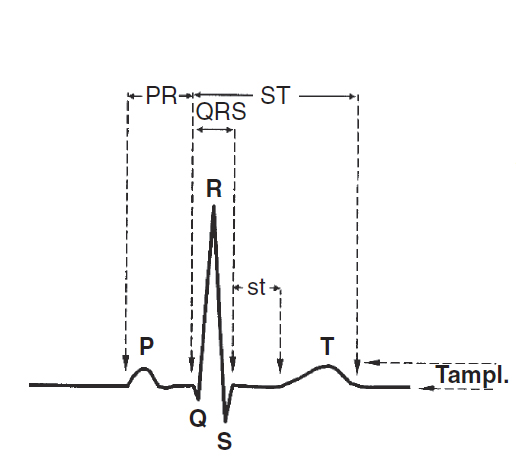
\includegraphics[width=100mm]{SinusRythmLabels.jpg}
    \caption{Sinus Rhythm Labels \cite{cacioppo_cardiovascular_2016_p_183_216}.}
    \label{fig:sinus_rhythm_labels}
\end{figure}

\subsection{QRS Complex}
The QRS Complex has a lot of clinical significance. The QRS complex is useful in diagnosing cardiac arrhythmias, conduction abnormalities, ventricular hypertrophy, myocardial infarction, electrolyte derangements, and other disease states \cite{noauthor_qrs_2018}.
\paragraph{}
The QRS Complex has also been utilized by several researchers to extract features to detect emotions. For example, \citeauthor{kim_emotion_2004}, were able to extract features in time and frequency domain to recognize emotions in music listening \cite{kim_emotion_2004}.

\subsection{R-R Interval}
\label{sec:rrinterval}
The R-R interval or the heart period is the time in \textit{msec} between peaks of two consecutive sinus rhythms. The heart period is converted into heat rate in beats/min or bpm using the equation \cite{cacioppo_cardiovascular_2016_p_183_216}. The variation of the heart rate over a certain period of time is called the Heart Rate Variability (HRV) \cite{noauthor_what_2017}.

\begin{equation}
\label{eq:hrv}
    HRV(beats/min) = \frac{60}{heart period (msec) \times 1000}
\end{equation}

\subsection{Emotions in Electrocardiogram}
The sinoatrial node which generates the sinus rhythm is modulated by the activity level of the Parasympathetic Nervous System (PNS) and the Sympathetic Nervous System (SNS). The Parasympathetic and the Sympathetic Nervous system are branches of the Autonomic Nervous System (ANS). Thus if the heartbeat is treated as a random point process, the heart rate is dependent on the activity of the Autonomic Nervous System (ANS), which is, in fact, dependent on emotional stimuli \cite{kim_emotion_2004}. The relation between the Parasympathetic and the Sympathetic nervous system with the Heart Period is shown in figure \ref{fig:ecg_emotions}.

\begin{figure}
    \centering
    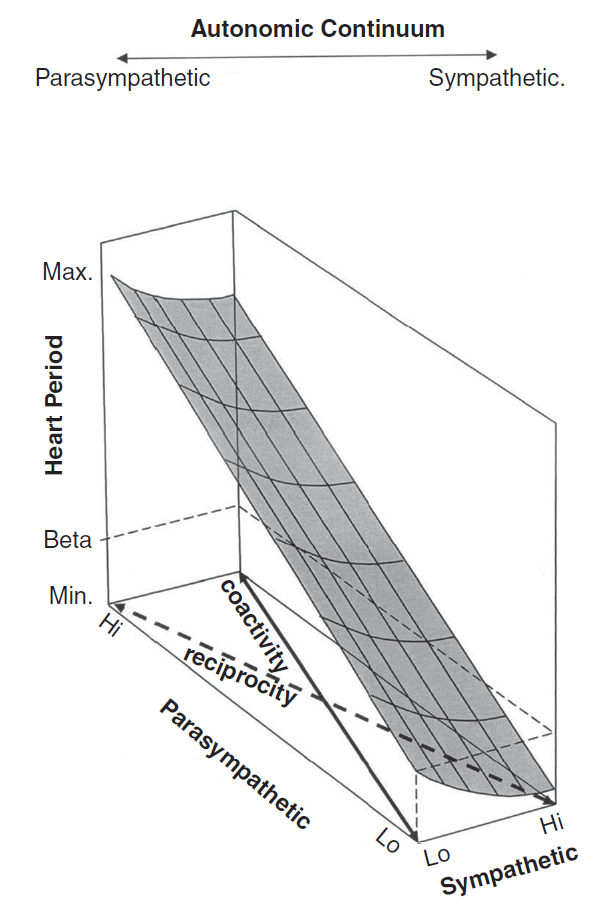
\includegraphics[width=100mm]{ecg_emotions.jpg}
    \caption{Cardiac Autonomic Space \cite{cacioppo_cardiovascular_2016_p_183_216}.}
    \label{fig:ecg_emotions}
\end{figure}

\subsection{Electrode Placement} 
\label{sec:einthoven} An electrode --- a wire cable --- connected to the patient are placed on different parts of the body in order to record the Electrocardiogram. The placement of electrodes in clinical electrocardiology is represented by Einthoven's triangle as shown in figure \ref{fig:einthoven_triangle}. In a 3-leads placement the electrodes are placed on right arm (aV\textsubscript{R}), left arm (aV\textsubscript{L}) and left leg (aV\textsubscript{F}). These leads are often approximated by electrode placement on the torso, rather than the limbs \cite{cacioppo_cardiovascular_2016_p_183_216}. To obtain better resolution of the Electrocardiogram signal a 12-leads placement is used for the clinical diagnosis. Sometimes leads and electrodes are used interchangeably. However, strictly speaking, a lead corresponds to the pattern generated within the sinus rhythm \cite{hampton_ecg_2013}. Thus the edges of the Einthoven's triangle in figure \ref{fig:einthoven_triangle} show the electrode placement. While the open arrows indicate electrical vectors associated with the lead patterns generated during P, Q and R waves of the ECG \cite{cacioppo_cardiovascular_2016_p_183_216}.

\begin{figure}
    \centering
    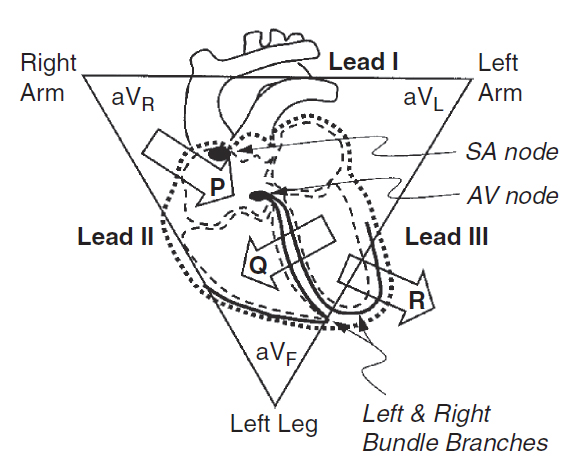
\includegraphics[width=100mm]{Figures/einthoven_triangle.jpg}
    \caption{Einthoven's triangle \cite{cacioppo_cardiovascular_2016_p_183_216}.}
    \label{fig:einthoven_triangle}
\end{figure}

\section{EDA}
The skin acts as a protective barrier which helps in maintaining core body temperature and water balance. This is regulated by variation in the production of sweat. There are two kinds of sweat glands in the human body, the apocrine and the eccrine. The apocrine glands open into the hair under the skin of the body while eccrine glands open on to the surface of the body. The eccrine have been the primary interest of psycho-physiologists. The eccrine are sweat glands that help in thermoregulation (maintaining core body temperature). The glands located on palmar and plantar surfaces, i.e. the surface of the palm and the feet respectively, are thought to be associated more with psychologically significant stimuli than thermal stimuli. Thus EDA has been widely been used in psychological studies \cite{cacioppo_electrodermal_2016_p_217_243}.

\subsection{Anatomy of the Eccrine Sweat Glands}
The anatomy of the eccrine sweat glands is shown in figure \ref{fig:eccrine_glands}. The eccrine sweat glands are a coiled compact body, the secretory portion of the gland. The eccrine sweat duct carries the sweat to the sweat pore. The sweat duct remains straight through the stratum Malpighi and stratum Lucidum; spirals through stratum corneum and opens on the surface of the skin \cite{cacioppo_electrodermal_2016_p_217_243}.
\begin{figure}
    \centering
    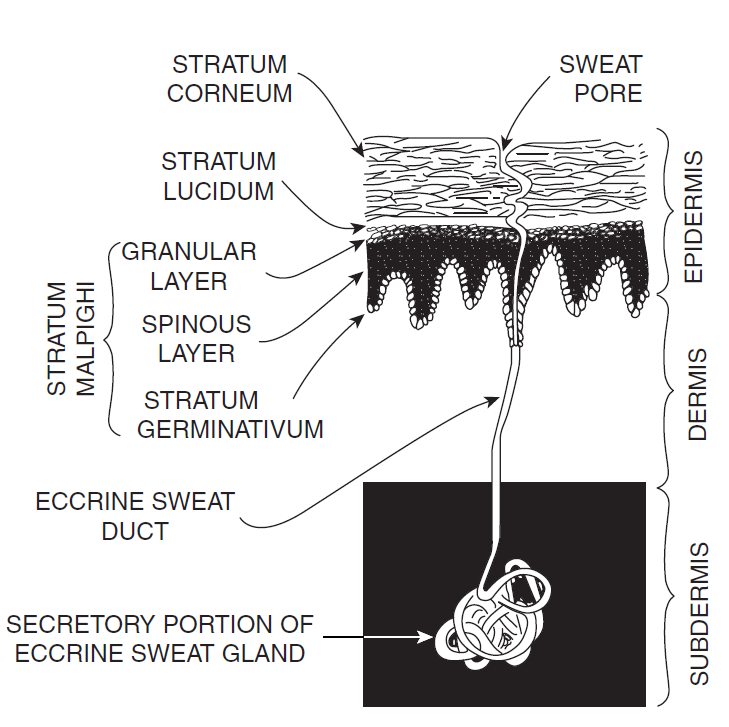
\includegraphics[width=100mm]{Figures/eccrine_glands.PNG}
    \caption{Anatomy of the eccrine sweat gland in various layer of skin \cite{hassett_primer_1978}.}
    \label{fig:eccrine_glands}
\end{figure}

\subsection{The correlation between Sweat Glands and EDA}
Depending on the degree of activation of the Sympathetic Nervous System (SNS) varying amount of sweat is secreted out of the sweat pores. If the sweat ducts are considered to be a set of variable resistors then an increase in sweat would increase the conductivity. The higher the amount of sweat, the lower the resistance between sweat ducts. Thus changes in the level of sweat in the sweat ducts yield an observable change in EDA \cite{cacioppo_electrodermal_2016_p_217_243}.

\subsection{Measuring EDA}
The EDA is usually measured by placing two electrodes on the palmar or the plantar surfaces. There are two methods to determine the change in EDA. The Alternating Current (AC) method, which is infrequently used and the Direct Current (DC) method, which is commonly used to measure skin conductance or skin resistance. The principle of Ohm's Law is utilized to measure skin conductance. Given a constant voltage (V) and an alternating skin resistance (R) the current passing through the skin (I) can be measured by I = V/R. The current flowing through the skin is reciprocal of skin resistance is called skin conductance which is a measure of EDA. Conductance is expressed in units of Siemens. Since the resistance of the skin is very high the skin conductance has much lower value. Hence, skin conductance is expressed in units of microSiemens ($\mu$S). \cite{cacioppo_electrodermal_2016_p_217_243}.

\subsection{Electrode Placement}
\label{sec:electrode_placement}
With the Direct Current (DC) recording method, the polarization of electrodes can happen. The polarization occurs as the impedance increases between the skin-electrode contact as the sweat accumulates overtime. This results in degradation of signal quality of EDA. Typically Silver-silver chloride (Ag/AgCl) electrodes are used to measure EDA as they minimize the development of bias potential and polarization. 

\paragraph{EDA Recording} The EDA is recorded by placing two electrodes on the surface of the skin. Numerous anatomical sites on the skin were examined by \citeauthor{culp_regional_1966} in 1966 to find the ideal placement for recording the EDA and it was found that the plantar surface of the foot to be ideal for recording EDA \cite{culp_regional_1966}. However, \citeauthor{van_dooren_emotional_2012} noticed that the placement of electrodes on the foot measured a lower EDA signals than electrode placement on the palms \cite{van_dooren_emotional_2012}. \citeauthor{payne_lapses_2016} found that the electrodes placement on the palm generated a comparable EDA to that of the  electrodes placed on the toe \cite{payne_lapses_2016}. Thus the reading is typically taken from active locations where sweat secretion is high for example the surface of the palms or the feet. The most common placements for palm are shown in the figure \ref{fig:eda_electrode_placement}. The direction of the electrodes does not matter since both the electrodes are placed on active sites where secretion of sweat is almost equal. However, not all the placements are shown in figure \ref{fig:eda_electrode_placement} result in the same level of conductance. The higher number of sweat glands present in position 1 gives a higher EDA reading than position 2 or position 3. Hence position 1 location should be used for recording unless there is a specific reason not to \cite{cacioppo_electrodermal_2016_p_217_243}.

\begin{figure}
    \centering
    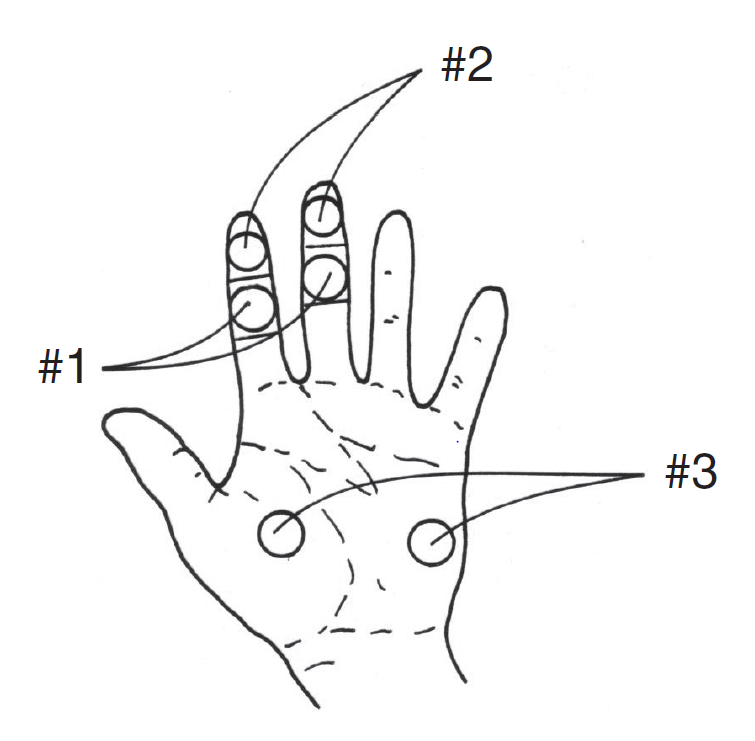
\includegraphics[width=100mm]{Figures/eda_electrode_placement.PNG}
    \caption{Three possible positions of electrode placement to record EDA \cite{cacioppo_electrodermal_2016_p_217_243}.}
    \label{fig:eda_electrode_placement}
\end{figure}

\begin{figure}
    \centering
    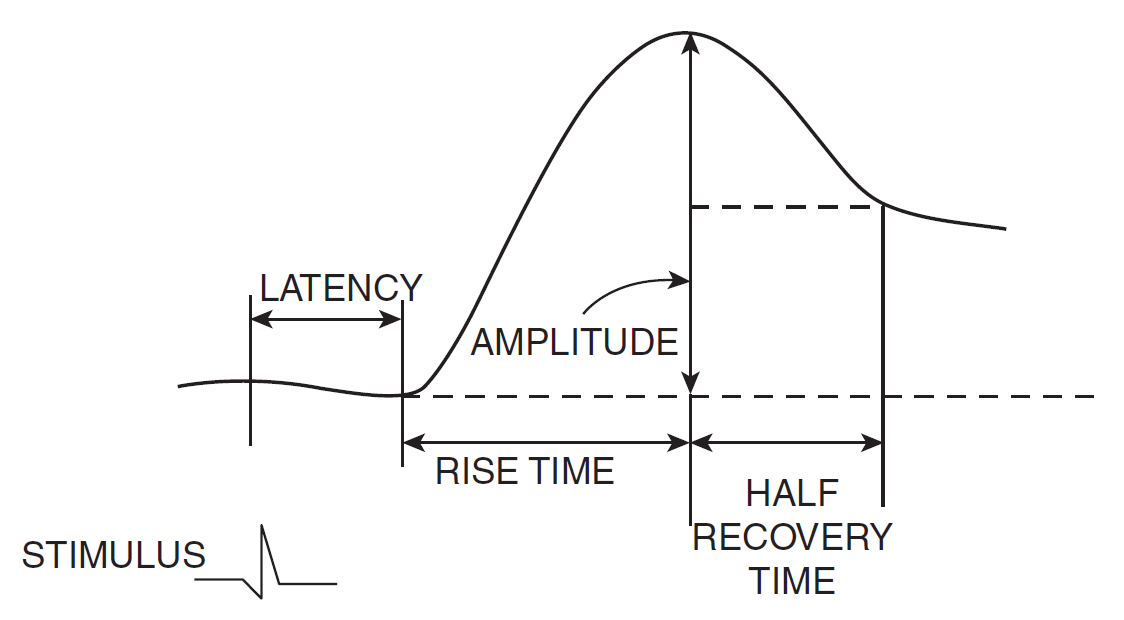
\includegraphics[width=100mm]{eda_response.PNG}
    \caption{Time-domain measures of EDA \cite{cacioppo_electrodermal_2016_p_217_243}.}
    \label{fig:eda_graph}
\end{figure}

\subsection{Quantifying EDA}
\label{sec:quantify_eda}
Figure \ref{fig:eda_graph} shows the quantification of skin conductance in the time domain when an external stimuli is applied. The moment at which the stimuli is applied is called \textbf{Onset}. The stimuli are followed by a short latency window of about 1-3s. Thereafter the response to the stimuli is triggered by an increase in skin conductance. Which in turn, increases EDA. This period between skin conductance initiation and the peak of 1-3s is called \textbf{Rise Time}. Following this period the skin conductance level decrease. The time period from the peak to the point of 50$\%$ recovery is called \textbf{Half Recovery Time}. The phasic increase in skin conductance level after initiation of a response to the peak is called \textbf{Amplitude}. The amplitude ranges between 0.2-1.0$\mu$S \cite{cacioppo_electrodermal_2016_p_217_243}.

\subsection{Tonic and Phasic EDA}
\label{sec:tonic_phasic_eda}
The time series plot of the skin conductance (SC) is a compound of slowly changing tonic activity and fast-changing phasic activity. The tonic activity is generally influenced by the internal changes in the body. The phasic activity reflects a stimuli specific response. The deconvolution using a driver function and the Impulse Response Function generalized as
$$SC = (Driver\textsubscript{tonic} + Driver\textsubscript{phasic})*IRF$$
The figure \ref{fig:phasic_tonic_eda} illustrates the skin conductance data section of 165s with four sections where stimuli were induced for 6,8,4 and 2s. The first graph shows the original skin conductance data. The dashed lines show the tonic skin conductance obtained using tonic driver function (inter-impulse data of 10s). The second graph shows the driver signal resulting from the deconvolution of the skin conductance data. Subtractions of the tonic part from the driver result in the phasic driver. The phasic driver has virtually zero baseline and distinct phasic responses after the stimuli is induced, shaded in black in third graph \cite{benedek_continuous_2010}.
\begin{figure}
    \centering
    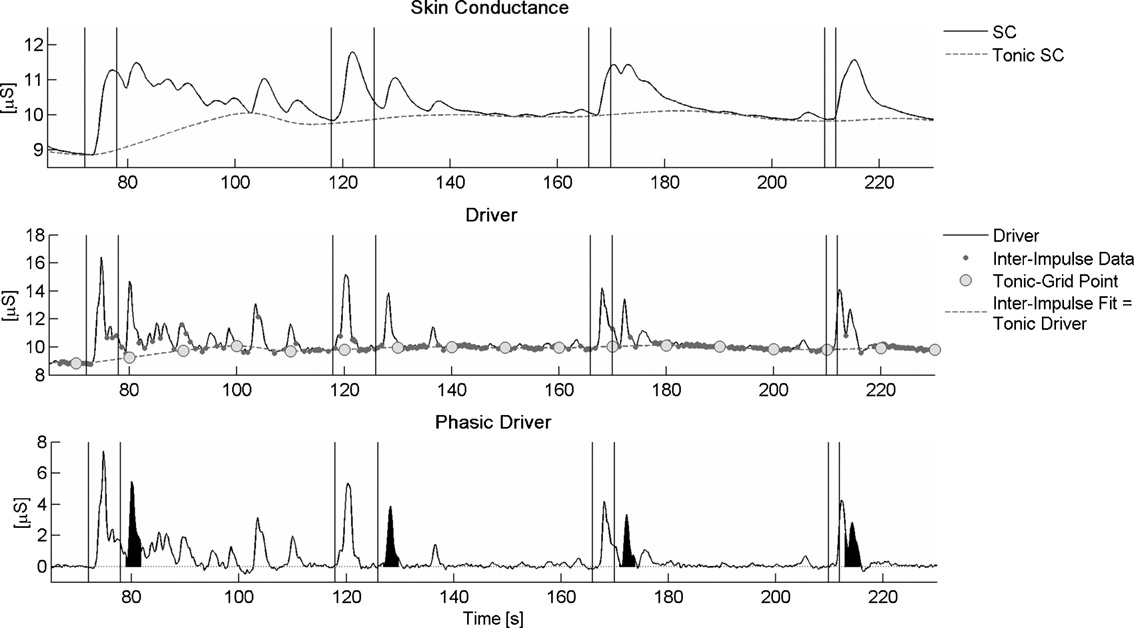
\includegraphics[width=150mm]{Figures/phasic_tonic_eda.jpg}
    \caption{Phasic and Tonic Driver extraction \cite{benedek_continuous_2010}.}
    \label{fig:phasic_tonic_eda}
\end{figure}


Figure \ref{fig:eda_graph} shows a typical time-domain measure of EDA due to Skin Conductance Response (SCR), because of instantaneous stimuli. The SCR’s stimulus-onset latency, amplitude and rise time are used to assess the level of stress induced by stimuli. 






